\documentclass[aspectratio=169,9pt]{beamer}

\usepackage{amsmath,amssymb}
\usepackage{booktabs,tabularx,array}
\usepackage{graphicx}
\usepackage{tikz}
\usetikzlibrary{arrows.meta,positioning,calc}
\usepackage[most]{tcolorbox}
\usepackage{microtype}
\usepackage{ragged2e}
\usepackage{lmodern}
\renewcommand{\familydefault}{\sfdefault}

% ---------- Palette ----------
\definecolor{bg}{HTML}{07111E}
\definecolor{panel}{HTML}{101C2E}
\definecolor{paneltwo}{HTML}{0C1727}
\definecolor{text}{HTML}{F5F7FB}
\definecolor{muted}{HTML}{AAB6C8}
\definecolor{cyan}{HTML}{45D7FF}
\definecolor{violet}{HTML}{A78BFA}
\definecolor{green}{HTML}{4CE19B}
\definecolor{amber}{HTML}{FFCA5C}
\definecolor{red}{HTML}{FF7183}
\definecolor{line}{HTML}{263750}

% ---------- Beamer ----------
\setbeamercolor{normal text}{fg=text,bg=bg}
\setbeamercolor{frametitle}{fg=text,bg=bg}
\setbeamercolor{structure}{fg=cyan}
\setbeamercolor{itemize item}{fg=cyan}
\setbeamercolor{itemize subitem}{fg=violet}
\setbeamertemplate{navigation symbols}{}
\setbeamertemplate{itemize item}{\raise0.2ex\hbox{\tiny$\blacktriangleright$}}
\setbeamertemplate{itemize subitem}{\raise0.15ex\hbox{\tiny$\bullet$}}
\setbeamersize{text margin left=0.52cm,text margin right=0.52cm}
\setbeamerfont{frametitle}{size=\Large,series=\bfseries}
\setbeamerfont{title}{size=\fontsize{24}{27}\selectfont,series=\bfseries}
\setbeamerfont{subtitle}{size=\large}
\setlength{\abovedisplayskip}{3.5pt}
\setlength{\belowdisplayskip}{3.5pt}
\setlength{\abovedisplayshortskip}{2pt}
\setlength{\belowdisplayshortskip}{2pt}

\setbeamertemplate{frametitle}{%
  \vspace{0.08cm}%
  \begin{beamercolorbox}[wd=\paperwidth,ht=0.56cm,dp=0.08cm,leftskip=0.52cm]{frametitle}
  \insertframetitle
  \end{beamercolorbox}%
  \vspace{-0.04cm}\hspace{0.52cm}{\color{line}\rule{14.78cm}{0.45pt}}
}

\setbeamertemplate{footline}{%
  \leavevmode\hbox{%
  \begin{beamercolorbox}[wd=.84\paperwidth,ht=.22cm,dp=.10cm,leftskip=.52cm]{author in head/foot}
    {\color{muted}\fontsize{5.8}{6.8}\selectfont SLIM — reproduction, diagnosis, extensions}
  \end{beamercolorbox}%
  \begin{beamercolorbox}[wd=.16\paperwidth,ht=.22cm,dp=.10cm,rightskip=.52cm plus1fil]{date in head/foot}
    {\color{muted}\fontsize{5.8}{6.8}\selectfont \insertframenumber/15}
  \end{beamercolorbox}}
}

% ---------- Helpers ----------
\newcommand{\hilite}[1]{\textcolor{cyan}{\textbf{#1}}}
\newcommand{\vio}[1]{\textcolor{violet}{\textbf{#1}}}
\newcommand{\good}[1]{\textcolor{green}{\textbf{#1}}}
\newcommand{\warn}[1]{\textcolor{amber}{\textbf{#1}}}
\newcommand{\bad}[1]{\textcolor{red}{\textbf{#1}}}
\newcommand{\tinycite}[1]{{\color{muted}\fontsize{5.7}{6.7}\selectfont #1}}

\newtcolorbox{darkbox}[1][]{enhanced,colback=panel,colframe=line,coltext=text,
  boxrule=.45pt,arc=1.8mm,left=1.8mm,right=1.8mm,top=1.3mm,bottom=1.3mm,#1}
\newtcolorbox{cyanbox}[1][]{enhanced,colback=paneltwo,colframe=cyan,coltext=text,
  boxrule=.75pt,arc=1.8mm,left=1.8mm,right=1.8mm,top=1.3mm,bottom=1.3mm,#1}
\newtcolorbox{violetbox}[1][]{enhanced,colback=paneltwo,colframe=violet,coltext=text,
  boxrule=.75pt,arc=1.8mm,left=1.8mm,right=1.8mm,top=1.3mm,bottom=1.3mm,#1}
\newtcolorbox{greenbox}[1][]{enhanced,colback=paneltwo,colframe=green,coltext=text,
  boxrule=.75pt,arc=1.8mm,left=1.8mm,right=1.8mm,top=1.3mm,bottom=1.3mm,#1}
\newcommand{\tagg}[2]{\tikz[baseline=(X.base)]\node[rounded corners=1.1mm,inner xsep=1.2mm,inner ysep=.45mm,fill=#1!15,draw=#1!65,text=#1,font=\fontsize{5.8}{6.5}\selectfont\bfseries] (X) {#2};}

\title{SLIM: Sparsified Late Interaction for Multi-Vector Retrieval}
\subtitle{Reproduction $\rightarrow$ Diagnosis $\rightarrow$ Extensions}
\author{Harshit Raj \quad \textbullet \quad Team members}
\institute{Information Retrieval Project, IIT Bombay}
\date{October 2026}

\begin{document}

% ------------------------------------------------------------------
\begin{frame}[plain]
\begin{tikzpicture}[remember picture,overlay]
  \fill[bg] (current page.south west) rectangle (current page.north east);
  % \fill[cyan!8] ([xshift=12.6cm,yshift=-.8cm]current page.north west) circle (2.4cm);
  % \fill[violet!8] ([xshift=14.3cm,yshift=-1.5cm]current page.north west) circle (1.75cm);
\end{tikzpicture}
\vspace{0.45cm}
{\color{cyan}\small\bfseries INFORMATION RETRIEVAL PROJECT}\par
\vspace{0.25cm}
{\usebeamerfont{title}\color{text}\inserttitle\par}
\vspace{0.12cm}
{\usebeamerfont{subtitle}\color{muted}\insertsubtitle\par}
\vspace{0.45cm}
\begin{columns}[T,totalwidth=\textwidth]
\column{0.46\textwidth}
\begin{darkbox}
\small
\textbf{Core question.} Can we keep the fine-grained accuracy of \hilite{token-level late interaction} while moving candidate generation back to a standard \hilite{inverted index}?
\end{darkbox}
\vspace{0.2cm}
{\small\color{muted}\insertauthor\\\insertinstitute}

\column{0.50\textwidth}
\centering
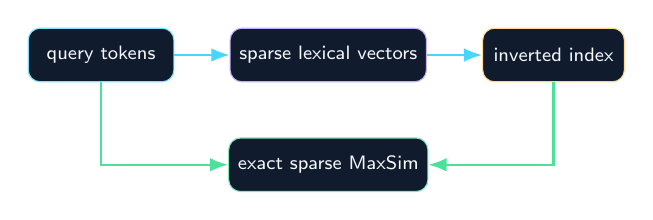
\begin{tikzpicture}[node distance=5mm,>=Latex,every node/.style={font=\scriptsize}]
\node[rounded corners=1.5mm,draw=cyan!70,fill=panel,minimum width=1.85cm,minimum height=.68cm,text=text] (q) {query tokens};
\node[rounded corners=1.5mm,draw=violet!70,fill=panel,minimum width=2.2cm,minimum height=.68cm,text=text,right=7mm of q] (s) {sparse lexical vectors};
\node[rounded corners=1.5mm,draw=amber!70,fill=panel,minimum width=1.8cm,minimum height=.68cm,text=text,right=7mm of s] (i) {inverted index};
\node[rounded corners=1.5mm,draw=green!70,fill=panel,minimum width=2.05cm,minimum height=.68cm,text=text,below=7mm of s] (m) {exact sparse MaxSim};
\draw[->,thick,cyan] (q)--(s);
\draw[->,thick,cyan] (s)--(i);
\draw[->,thick,green] (i.south) |- (m.east);
\draw[->,thick,green] (q.south) |- (m.west);
\end{tikzpicture}
\end{columns}
\vfill
\tinycite{Primary paper: Li et al., “SLIM: Sparsified Late Interaction for Multi-Vector Retrieval with Inverted Indexes”, SIGIR 2023.}
\end{frame}

% ------------------------------------------------------------------
\begin{frame}[t]{1. Why SLIM exists}
\begin{columns}[T,totalwidth=\textwidth]
\column{0.31\textwidth}
\begin{darkbox}
{\color{amber}\bfseries Sparse single-vector retrieval}\par\smallskip
\small BM25/SPLADE compress each document to one lexical vector.
\begin{itemize}\scriptsize
\item Excellent inverted-index compatibility.
\item Cheap first-stage retrieval.
\item But token-level matching structure is compressed away.
\end{itemize}
\end{darkbox}

\column{0.31\textwidth}
\begin{darkbox}
{\color{violet}\bfseries Dense late interaction}\par\smallskip
\small ColBERT preserves a vector per token and scores
\[
S(q,d)=\sum_i\max_j q_i^\top d_j.
\]
\begin{itemize}\scriptsize
\item Fine-grained token-to-token evidence.
\item Much heavier multi-vector indexing/search.
\end{itemize}
\end{darkbox}

\column{0.34\textwidth}
\begin{cyanbox}
{\color{cyan}\bfseries SLIM's compromise}\par\smallskip
\small Contextual token embeddings are projected into a shared, \textbf{non-negative sparse lexical space}.
\begin{itemize}\scriptsize
\item sparse token vectors preserve MaxSim refinement;
\item document max-pooling produces one Lucene-indexable vector;
\item candidate generation is approximate, refinement is exact under the sparse model.
\end{itemize}
\end{cyanbox}
\end{columns}
\vspace{0.12cm}
\begin{darkbox}
\small \textbf{The actual research question is not “sparse vs dense”.} It is whether a \hilite{single-vector sparse first stage} can preserve enough of the candidates required by an \vio{exact token-level second stage}.
\end{darkbox}
\end{frame}

% ------------------------------------------------------------------
\begin{frame}[t]{2. SLIM in one slide — the paper's architecture}
\begin{columns}[T,totalwidth=\textwidth]
\column{0.63\textwidth}
\begin{darkbox}
\centering
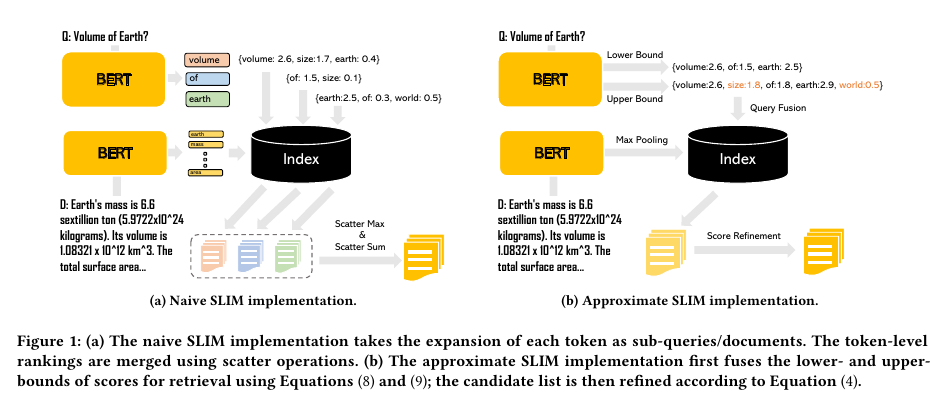
\includegraphics[width=.97\linewidth,height=5.1cm,keepaspectratio]{slim_fig1.png}
\end{darkbox}
\column{0.34\textwidth}
\begin{cyanbox}
\scriptsize
\textbf{1. Sparse contextual tokens}\par
BERT + MLM projection maps each token into a sparse vector over the vocabulary.
\end{cyanbox}
\vspace{0.10cm}
\begin{violetbox}
\scriptsize
\textbf{2. One-vector candidate retrieval}\par
Document token vectors are max-pooled; query-side lower/upper-bound representations are fused into one sparse query vector.
\end{violetbox}
\vspace{0.10cm}
\begin{greenbox}
\scriptsize
\textbf{3. Exact sparse late interaction}\par
For the retrieved candidates, the original sparse token vectors are loaded and Eq. 4 is recomputed exactly.
\end{greenbox}
\vspace{0.08cm}
\tinycite{Figure reproduced from the SLIM paper, Fig. 1.}
\end{columns}
\end{frame}

% ------------------------------------------------------------------
\begin{frame}[t]{3. The mathematics that makes SLIM indexable}
\begin{columns}[T,totalwidth=\textwidth]
\column{0.49\textwidth}
\begin{darkbox}
\scriptsize
\textbf{Sparse lexical projection.} For contextual token embedding $v_{d_j}$:
\[
\phi_{d_j}=\log\!\left(1+\operatorname{ReLU}(W^\top v_{d_j}+b)\right)
\in \mathbb{R}_{\ge0}^{|V|}.
\]
The same mapping gives query token vectors $\phi_{q_i}$.
\end{darkbox}
\vspace{0.10cm}
\begin{cyanbox}
\scriptsize
\textbf{Exact sparse late interaction (paper Eq. 4)}
\[
S(q,d)=\sum_{i=1}^{N}\max_{1\le j\le M}\phi_{q_i}^{\top}\phi_{d_j}.
\]
The scorer is still MaxSim. The difference is that each token vector is now sparse and lexical.
\end{cyanbox}

\column{0.48\textwidth}
\begin{darkbox}
\scriptsize
Define the document max-pool
\[
D_d=\max_j \phi_{d_j}\quad\text{(elementwise)}.
\]
For each query token keep only its largest lexical coordinate, giving $e_{q_i}$. Then the paper derives
\[
L(q,d)=\Big(\sum_i e_{q_i}\Big)^\top D_d
\le S(q,d)\le
\Big(\sum_i\phi_{q_i}\Big)^\top D_d=U(q,d).
\]
\end{darkbox}
\vspace{0.10cm}
\begin{violetbox}
\scriptsize
\textbf{First-stage proxy (paper Eq. 9)}
\[
A_\beta(q,d)=\beta L(q,d)+(1-\beta)U(q,d)
\]
\[
=\Big[\sum_i\big(\beta e_{q_i}+(1-\beta)\phi_{q_i}\big)\Big]^\top D_d.
\]
So first-stage ranking becomes \vio{one sparse dot product per document}.
\end{violetbox}
\end{columns}
\vspace{0.08cm}
\tinycite{Li et al., Sec. 2; non-negativity is what makes the lower/upper-bound argument work.}
\end{frame}

% ------------------------------------------------------------------
\begin{frame}[t]{4. What actually happens at indexing and retrieval time}
\begin{columns}[T,totalwidth=\textwidth]
\column{0.49\textwidth}
\centering
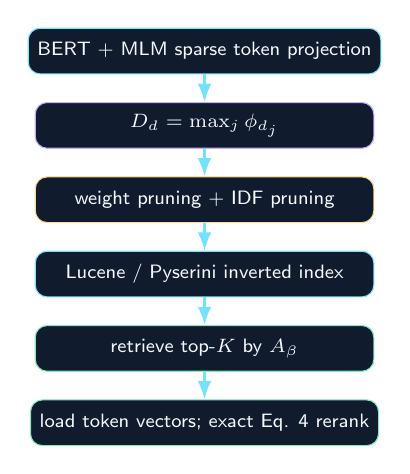
\begin{tikzpicture}[node distance=3.5mm,>=Latex,every node/.style={font=\scriptsize}]
\node[rounded corners=1.5mm,draw=cyan!70,fill=panel,text=text,minimum width=4.3cm,minimum height=.58cm] (a) {BERT + MLM sparse token projection};
\node[rounded corners=1.5mm,draw=violet!70,fill=panel,text=text,minimum width=4.3cm,minimum height=.58cm,below=of a] (b) {$D_d=\max_j \phi_{d_j}$};
\node[rounded corners=1.5mm,draw=amber!70,fill=panel,text=text,minimum width=4.3cm,minimum height=.58cm,below=of b] (c) {weight pruning + IDF pruning};
\node[rounded corners=1.5mm,draw=cyan!70,fill=panel,text=text,minimum width=4.3cm,minimum height=.58cm,below=of c] (d) {Lucene / Pyserini inverted index};
\node[rounded corners=1.5mm,draw=green!70,fill=panel,text=text,minimum width=4.3cm,minimum height=.58cm,below=of d] (e) {retrieve top-$K$ by $A_\beta$};
\node[rounded corners=1.5mm,draw=green!70,fill=panel,text=text,minimum width=4.3cm,minimum height=.58cm,below=of e] (f) {load token vectors; exact Eq. 4 rerank};
\foreach \u/\v in {a/b,b/c,c/d,d/e,e/f}{\draw[->,thick,cyan!75] (\u)--(\v);}
\end{tikzpicture}

\column{0.48\textwidth}
\begin{darkbox}
\scriptsize
\textbf{Paper default configuration}
\begin{itemize}\scriptsize
\item token-weight threshold: $0.5$;
\item IDF threshold: $3$;
\item fusion coefficient: $\beta=0.01$;
\item Pyserini/Lucene first stage retrieves top $4000$;
\item exact sparse late-interaction refinement outputs top $1000$.
\end{itemize}
\end{darkbox}
\vspace{0.10cm}
\begin{cyanbox}
\scriptsize
\textbf{Two different stored objects matter.} Lucene only needs the pooled $D_d$ vectors. Exact refinement additionally needs the surviving \emph{token-level sparse vectors}; those are stored separately.
\end{cyanbox}
\vspace{0.10cm}
\begin{violetbox}
\scriptsize
This separation is the central systems idea: candidate generation is engineered for inverted-index efficiency, while the second stage retains the richer token interaction.
\end{violetbox}
\end{columns}
\end{frame}

% ------------------------------------------------------------------
\begin{frame}[t]{5. What the original paper actually evaluates}
\begin{columns}[T,totalwidth=\textwidth]
\column{0.58\textwidth}
\begin{darkbox}
\centering
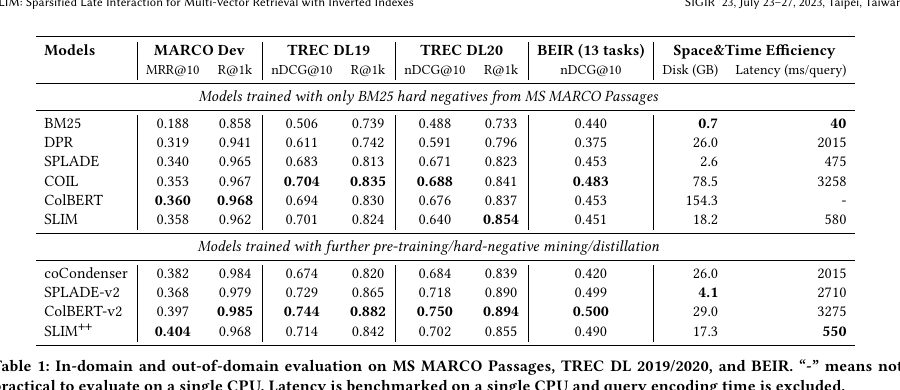
\includegraphics[width=.98\linewidth,height=3.35cm,keepaspectratio]{slim_table1.png}
\end{darkbox}
\vspace{0.08cm}
\begin{darkbox}
\centering
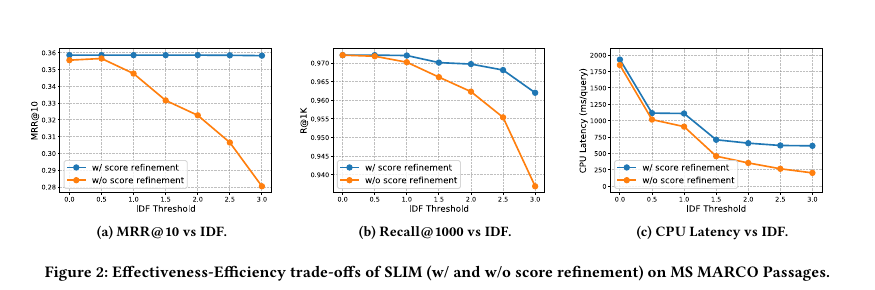
\includegraphics[width=.98\linewidth,height=1.75cm,keepaspectratio]{slim_fig2.png}
\end{darkbox}
\column{0.39\textwidth}
\begin{cyanbox}
\scriptsize
\textbf{Benchmarks / metrics}
\begin{itemize}\scriptsize
\item MS MARCO Passage dev: MRR@10, Recall@1K;
\item TREC DL19/20: nDCG@10 and recall;
\item 13 BEIR tasks: average nDCG@10.
\end{itemize}
\end{cyanbox}
\vspace{0.08cm}
\begin{darkbox}
\scriptsize
\textbf{Headline numbers.} SLIM reports MRR@10 $0.358$; SLIM++ reports $0.404$. SLIM++ also reports BEIR avg. nDCG@10 $0.490$, 17.3 GB index size, and 550 ms/query CPU latency in the authors' setup.
\end{darkbox}
\vspace{0.08cm}
\begin{violetbox}
\scriptsize
\textbf{Most informative experiment.} The authors vary IDF pruning and candidate depth. Exact refinement recovers much of the ranking quality lost by a cheaper first stage; the paper reports a large latency reduction for only a small MRR/recall drop.
\end{violetbox}
\vspace{0.05cm}
\tinycite{Top: Table 1. Bottom: Fig. 2, SLIM paper.}
\end{columns}
\end{frame}

% ------------------------------------------------------------------
\begin{frame}[t]{6. Our reproduction pipeline — what must match before numbers are meaningful}
\centering

\begin{tikzpicture}[x=1cm,y=1cm,>=Latex,every node/.style={font=\fontsize{6.5}{7.2}\selectfont\bfseries}]
\node[rounded corners=1.2mm,draw=cyan!70,fill=panel,text=text,minimum width=1.65cm,minimum height=.52cm] (a) at (0,0) {Checkpoint};
\node[rounded corners=1.2mm,draw=violet!70,fill=panel,text=text,minimum width=1.65cm,minimum height=.52cm] (b) at (2.35,0) {Corpus encode};
\node[rounded corners=1.2mm,draw=amber!70,fill=panel,text=text,minimum width=1.65cm,minimum height=.52cm] (c) at (4.7,0) {Prune + pool};
\node[rounded corners=1.2mm,draw=cyan!70,fill=panel,text=text,minimum width=1.65cm,minimum height=.52cm] (d) at (7.05,0) {Lucene index};
\node[rounded corners=1.2mm,draw=green!70,fill=panel,text=text,minimum width=1.65cm,minimum height=.52cm] (e) at (9.4,0) {Top-$K$};
\node[rounded corners=1.2mm,draw=green!70,fill=panel,text=text,minimum width=1.65cm,minimum height=.52cm] (f) at (11.75,0) {Exact refine};
\node[rounded corners=1.2mm,draw=violet!70,fill=panel,text=text,minimum width=1.65cm,minimum height=.52cm] (g) at (14.1,0) {Evaluate};
\foreach \u/\v in {a/b,b/c,c/d,d/e,e/f,f/g}{\draw[->,thick,cyan!75] (\u)--(\v);}
\end{tikzpicture}
\vspace{0.28cm}
\begin{columns}[T,totalwidth=\textwidth]
\column{0.48\textwidth}
\begin{cyanbox}
\scriptsize
\textbf{Pipeline being reproduced}
\begin{itemize}\scriptsize
\item released SLIM/SLIM++ checkpoint and encoder;
\item sparse corpus token generation;
\item document max-pooling + post-hoc pruning;
\item Pyserini/Lucene candidate retrieval;
\item exact sparse token refinement;
\item MS MARCO effectiveness + efficiency measurements.
\end{itemize}
\end{cyanbox}
\column{0.49\textwidth}
\begin{darkbox}
\scriptsize
\textbf{Controls needed for a fair comparison}
\begin{itemize}\scriptsize
\item SLIM vs SLIM++ checkpoint;
\item token threshold, IDF threshold, $\beta$;
\item $K$ and whether refinement is enabled;
\item Pyserini/Lucene version and index settings;
\item CPU, thread count, batching, cache state;
\item whether query encoding is included in latency.
\end{itemize}
\end{darkbox}
\end{columns}
\vspace{0.12cm}
\begin{darkbox}
\centering\scriptsize \warn{Replace this line tonight with one precise sentence describing exactly what has already run successfully.}
\end{darkbox}
\end{frame}

% ------------------------------------------------------------------
\begin{frame}[t]{7. Reproduction result I — effectiveness}
\begin{columns}[T,totalwidth=\textwidth]
\column{0.56\textwidth}
\begin{darkbox}
\scriptsize
\textbf{Paper vs. our run}\par\smallskip
\renewcommand{\arraystretch}{1.18}
\begin{tabularx}{\linewidth}{>{\raggedright\arraybackslash}Xcc}
\toprule
Metric & Paper & Ours \\
\midrule
MS MARCO MRR@10 & 0.358 / 0.404 & \textcolor{amber}{[INSERT]} \\
MS MARCO Recall@1K & 0.962 / 0.968 & \textcolor{amber}{[INSERT]} \\
TREC DL19 nDCG@10 & 0.701 / 0.714 & \textcolor{amber}{[INSERT]} \\
TREC DL20 nDCG@10 & 0.640 / 0.702 & \textcolor{amber}{[INSERT]} \\
BEIR avg. nDCG@10 & 0.451 / 0.490 & \textcolor{amber}{[INSERT]} \\
\bottomrule
\end{tabularx}
\smallskip
{\color{muted}\fontsize{5.8}{6.6}\selectfont Paper values shown as SLIM / SLIM++ where both are reported.}
\end{darkbox}
\vspace{0.10cm}
\begin{violetbox}
\scriptsize
\textbf{One-line interpretation}\par
\textcolor{amber}{[e.g. “Matches the paper within X; the remaining gap is primarily first-stage candidate recall / refinement / configuration.”]}
\end{violetbox}

\column{0.41\textwidth}
\begin{cyanbox}
\scriptsize\textbf{Candidate recall vs. $K$}\par\smallskip
\centering
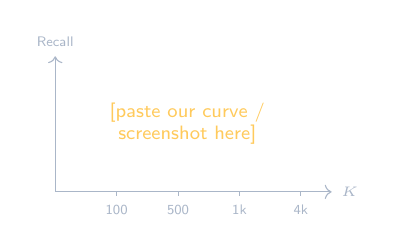
\begin{tikzpicture}[x=.78cm,y=.42cm]
\draw[->,muted] (0,0)--(4.5,0) node[right,font=\tiny,text=muted] {$K$};
\draw[->,muted] (0,0)--(0,4.1) node[above,font=\tiny,text=muted] {Recall};
\foreach \x/\lab in {1/100,2/500,3/1k,4/4k}{\draw[muted] (\x,0)--(\x,-.11) node[below,font=\tiny,text=muted]{\lab};}
\node[text=amber,font=\scriptsize,align=center] at (2.15,2.05) {[paste our curve /\\screenshot here]};
\end{tikzpicture}
\end{cyanbox}
\vspace{0.10cm}
\begin{darkbox}
\scriptsize
\textbf{Also report if available:} no-refinement score, refined score, and candidate recall. That immediately tells us whether a mismatch comes from candidate generation or reranking.
\end{darkbox}
\end{columns}
\end{frame}

% ------------------------------------------------------------------
\begin{frame}[t]{8. Reproduction result II — efficiency and diagnosis}
\begin{columns}[T,totalwidth=\textwidth]
\column{0.48\textwidth}
\begin{darkbox}
\scriptsize
\textbf{Efficiency numbers}\par\smallskip
\renewcommand{\arraystretch}{1.25}
\begin{tabularx}{\linewidth}{>{\raggedright\arraybackslash}Xcc}
\toprule
Metric & Paper & Ours \\
\midrule
Index size & 18.2 / 17.3 GB & \textcolor{amber}{[INSERT]} \\
Latency & 580 / 550 ms & \textcolor{amber}{[INSERT]} \\
Candidate depth $K$ & 4000 & \textcolor{amber}{[INSERT]} \\
Refinement & on & \textcolor{amber}{[INSERT]} \\
\bottomrule
\end{tabularx}
\end{darkbox}
\vspace{0.10cm}
\begin{cyanbox}
\scriptsize
\textbf{Observed bottleneck}\par
\textcolor{amber}{[INSERT 1–2 precise sentences: encoding / indexing / retrieval / refinement / I/O]}
\end{cyanbox}

\column{0.49\textwidth}
\begin{violetbox}
\scriptsize
\textbf{If our number differs, classify the reason}
\begin{itemize}\scriptsize
\item \textbf{Model/config:} checkpoint, threshold, $\beta$, $K$.
\item \textbf{Indexing:} Pyserini/Lucene version, pruning, quantization.
\item \textbf{Evaluation:} split or metric implementation.
\item \textbf{Systems:} CPU, threads, batching, warm/cold cache.
\end{itemize}
\end{violetbox}
\vspace{0.10cm}
\begin{darkbox}
\scriptsize
\textbf{Actual issue we encountered}\par
\textcolor{amber}{[INSERT exact error / mismatch / engineering issue, if any]}
\end{darkbox}
\vspace{0.10cm}
\begin{darkbox}
\scriptsize
\textbf{Diagnosis rule:} if effectiveness matches but latency does not, treat it as a systems/environment discrepancy—not a model failure.
\end{darkbox}
\end{columns}
\end{frame}

% ------------------------------------------------------------------
\begin{frame}[t]{9. What reproducing SLIM tells us about where to extend it}
\begin{columns}[T,totalwidth=\textwidth]
\column{0.49\textwidth}
\begin{darkbox}
\scriptsize \tagg{amber}{FIXED GLOBAL FUSION}\quad The paper uses one post-hoc $\beta$ for all queries/tokens. It is not trained to imitate the exact late-interaction ranking.
\end{darkbox}
\vspace{0.08cm}
\begin{darkbox}
\scriptsize \tagg{cyan}{FIXED CANDIDATE DEPTH}\quad The default system retrieves a fixed top-4000 even when an “easy” query may need far fewer candidates.
\end{darkbox}
\vspace{0.08cm}
\begin{darkbox}
\scriptsize \tagg{violet}{POST-HOC PRUNING}\quad Thresholds prune dimensions after training; the loss does not directly penalize long posting lists.
\end{darkbox}

\column{0.48\textwidth}
\begin{darkbox}
\scriptsize \tagg{green}{REFINEMENT STORAGE}\quad Exact second-stage scoring still retains document token vectors for candidates.
\end{darkbox}
\vspace{0.08cm}
\begin{cyanbox}
\scriptsize
\textbf{Design principle for our project.} Do not replace SLIM wholesale. Preserve the properties that make it attractive:
\begin{itemize}\scriptsize
\item non-negative sparse lexical representations;
\item standard inverted-index candidate retrieval;
\item exact sparse late-interaction refinement;
\item lightweight fine-tuning / offline processing only.
\end{itemize}
\end{cyanbox}
\vspace{0.08cm}
\begin{violetbox}
\scriptsize
The four extensions below each target one concrete source of cost or mismatch, and we separate \good{theorem-level guarantees} from \warn{empirical expectations}.
\end{violetbox}
\end{columns}
\end{frame}

% ------------------------------------------------------------------
\begin{frame}[t]{10. Extension 1 — certified adaptive candidate depth}
\begin{columns}[T,totalwidth=\textwidth]
\column{0.55\textwidth}
\begin{cyanbox}
\scriptsize
Use the true SLIM upper bound for candidate ordering:
\[
U(q,d)=\Big(\sum_i\phi_{q_i}\Big)^\top D_d,\qquad S(q,d)\le U(q,d).
\]
Retrieve the first $B$ documents by decreasing $U$. Let $\tau_k$ be the $k$-th largest \emph{exact} score among them and $\theta_B$ the $B$-th upper-bound score. Then
\[
\boxed{\tau_k\ge \theta_B\;\Longrightarrow\;\text{current top-}k\text{ is exact}.}
\]
\end{cyanbox}
\vspace{0.08cm}
\begin{darkbox}
\scriptsize
\textbf{Algorithm:} start $B=256$; exact-rerank; if the certificate fails, double $B$ ($512,1024,2048,\ldots$) until it passes.
\end{darkbox}

\column{0.42\textwidth}
\begin{greenbox}
\scriptsize
\tagg{green}{GUARANTEE}\par\smallskip
Every unseen document has $U(q,d)\le\theta_B$. Since $S(q,d)\le U(q,d)$, none can beat the current $k$-th exact score after $\tau_k\ge\theta_B$.
\end{greenbox}
\vspace{0.08cm}
\begin{violetbox}
\scriptsize
\textbf{Expected effect.} Easy queries stop after far fewer exact refinements; hard queries automatically spend more work. The goal is lower mean/p95 refinement cost without sacrificing top-$k$ correctness when certified.
\end{violetbox}
\vspace{0.08cm}
\begin{darkbox}
\scriptsize
\textbf{Caveat.} The mathematical bound must survive pruning and score quantization. We therefore validate first on an unpruned/conservative score path, then add safe accounting for omitted mass if necessary.
\end{darkbox}
\end{columns}
\end{frame}

% ------------------------------------------------------------------
\begin{frame}[t]{11. Extension 2 — lossless dominance pruning of document tokens}
\begin{columns}[T,totalwidth=\textwidth]
\column{0.54\textwidth}
\begin{cyanbox}
\scriptsize
Let $x_r,x_s\in\mathbb{R}_{\ge0}^{|V|}$ be two sparse token vectors from the same document. If
\[
x_r\le x_s \qquad\text{coordinatewise},
\]
then for every legal SLIM query token $q\ge0$,
\[
q^\top x_r\le q^\top x_s.
\]
Therefore $x_r$ can never be a unique MaxSim winner and may be deleted.
\end{cyanbox}
\vspace{0.08cm}
\begin{greenbox}
\scriptsize
\tagg{green}{EXACT PRESERVATION}\par\smallskip
Deleting $x_r$ leaves $\max_j q^\top x_j$ unchanged for every non-negative $q$; therefore the complete exact SLIM score is unchanged for every query.
\end{greenbox}

\column{0.43\textwidth}
\begin{violetbox}
\scriptsize
\textbf{Stage 1 is preserved too.} Because $x_r[k]\le x_s[k]$ for every coordinate $k$, removing $x_r$ cannot change
\[
D_d=\max_j x_j.
\]
So both the Lucene representation and the exact refinement score remain identical.
\end{violetbox}
\vspace{0.08cm}
\begin{darkbox}
\scriptsize
\textbf{Offline implementation}
\begin{enumerate}\scriptsize
\item sparse pairwise dominance tests inside each document;
\item remove certified dominated tokens before writing the refinement token store;
\item optional stronger convex-dominance test only if pairwise pruning is too weak.
\end{enumerate}
\end{darkbox}
\vspace{0.08cm}
\begin{darkbox}
\scriptsize
\textbf{Only empirical question:} how many tokens are actually removable, and whether the offline test is worth its preprocessing time.
\end{darkbox}
\end{columns}
\end{frame}

% ------------------------------------------------------------------
\begin{frame}[t]{12. Extension 3 — train for posting cost, not only sparsity}
\begin{columns}[T,totalwidth=\textwidth]
\column{0.55\textwidth}
\begin{darkbox}
\scriptsize
SLIM uses sparsity regularization and post-hoc IDF pruning. But equal nonzero counts can have very different retrieval cost: activating a dimension with a huge document frequency creates a much longer posting traversal.
\end{darkbox}
\vspace{0.08cm}
\begin{cyanbox}
\scriptsize
Apply the cost regularizer to the \emph{pooled vector Lucene actually indexes}. For batch $\mathcal B$:
\[
p_k=\frac{1}{|\mathcal B|}\sum_{d\in\mathcal B}D_d^{(k)},
\qquad c_k=\log(1+\mathrm{DF}_k),
\]
\[
\mathcal L_{DF}=\sum_k c_k p_k^2,
\qquad
\mathcal L=\mathcal L_{rank}+\alpha\mathcal L_{sparse}+\gamma\mathcal L_{DF}.
\]
\end{cyanbox}

\column{0.42\textwidth}
\begin{violetbox}
\scriptsize
\textbf{Why this is aligned with the engine.} The penalty is larger precisely on dimensions that create expensive long postings. It targets the representation entering Lucene rather than an abstract token-level nnz count.
\end{violetbox}
\vspace{0.08cm}
\begin{darkbox}
\scriptsize
\textbf{Feasible training plan.} Start from the released checkpoint, fine-tune briefly with the same ranking objective, sweep only a small set of $\gamma$, and plot MRR/nDCG against postings traversed, latency and index size.
\end{darkbox}
\vspace{0.08cm}
\begin{darkbox}
\scriptsize
\tagg{amber}{EMPIRICAL}\quad Expected: fewer expensive postings and a better latency/index-size frontier. No theorem guarantees unchanged effectiveness; this is a controlled Pareto trade-off.
\end{darkbox}
\end{columns}
\end{frame}

% ------------------------------------------------------------------
\begin{frame}[t]{13. Extension 4 — importance weighting + retrieval-aware query fusion}
\begin{columns}[T,totalwidth=\textwidth]
\column{0.56\textwidth}
\begin{cyanbox}
\scriptsize
Assign each query token a non-negative importance $w_i$:
\[
S_w(q,d)=\sum_i w_i\max_j\phi_{q_i}^\top\phi_{d_j},\qquad w_i\ge0.
\]
The bound survives immediately:
\[
\Big(\sum_iw_i e_{q_i}\Big)^\top D_d
\le S_w(q,d)\le
\Big(\sum_iw_i\phi_{q_i}\Big)^\top D_d.
\]
\end{cyanbox}
\vspace{0.08cm}
\begin{violetbox}
\scriptsize
Replace one global $\beta$ by token-adaptive $\lambda_i\in[0,1]$:
\[
R(q)=\sum_iw_i\left[\lambda_i e_{q_i}+(1-\lambda_i)\phi_{q_i}\right],
\qquad A(q,d)=R(q)^\top D_d.
\]
The first stage remains one Lucene-compatible sparse query vector.
\end{violetbox}

\column{0.41\textwidth}
\begin{darkbox}
\scriptsize
\textbf{Minimal model.} With contextual query embedding $h_i$:
\[
w_i=\operatorname{softplus}(a^\top h_i+b),\qquad
\lambda_i=\sigma(c^\top h_i+d).
\]
Freeze the SLIM encoder and train only these tiny heads.
\end{darkbox}
\vspace{0.08cm}
\begin{darkbox}
\scriptsize
\textbf{Teacher objective.} Distill ranking differences from exact SLIM:
\[
\mathcal L_{m}=\big[(A^+-A^-)-(S^+-S^-)\big]^2,
\]
optionally plus a listwise KL term over a small candidate set.
\end{darkbox}
\vspace{0.08cm}
\begin{darkbox}
\scriptsize
\tagg{amber}{EMPIRICAL}\quad Success criterion: higher exact-top-$k$ candidate recall at smaller $K$; not merely a better surrogate loss.
\end{darkbox}
\end{columns}
\end{frame}

% ------------------------------------------------------------------
\begin{frame}[t]{14. Execution plan, ablations, and what success means}
\begin{columns}[T,totalwidth=\textwidth]
\column{0.24\textwidth}
\begin{cyanbox}
\scriptsize
\textbf{1. Lock baseline}\par\smallskip
Match checkpoint/config, fill Slides 7–8, verify candidate recall vs. $K$.
\par\smallskip
\tagg{cyan}{STOP/GO}\quad No extension training until this is stable.
\end{cyanbox}

\column{0.24\textwidth}
\begin{greenbox}
\scriptsize
\textbf{2. Guaranteed ideas}\par\smallskip
Implement dominance pruning + adaptive-$K$ certification first.
\par\smallskip
\tagg{green}{LOW RISK}\quad Check exact score/ranking agreement.
\end{greenbox}

\column{0.24\textwidth}
\begin{darkbox}
\scriptsize
\textbf{3. Learned efficiency}\par\smallskip
DF-aware fine-tune; compare MRR/nDCG/Recall to postings, latency, storage.
\par\smallskip
\tagg{amber}{PARETO}\quad Keep only if frontier improves.
\end{darkbox}

\column{0.24\textwidth}
\begin{violetbox}
\scriptsize
\textbf{4. Query adaptation}\par\smallskip
Train $w_i,\lambda_i$ heads only after candidate-recall curves are reliable.
\par\smallskip
\tagg{violet}{ABLATION}\quad global $\beta$ vs adaptive $\lambda_i$.
\end{violetbox}
\end{columns}
\vspace{0.12cm}
\begin{darkbox}
\scriptsize
\textbf{Evaluation.} MS MARCO dev + TREC DL19/20; BEIR if time permits. Report MRR/nDCG/Recall, candidate recall vs. $K$, mean/p95 latency, postings traversed, Lucene index size and token-store size. For guaranteed methods, additionally verify \textbf{100\% score/top-$k$ agreement} against the unmodified model under the stated assumptions.
\end{darkbox}
\vspace{0.14cm}
\centering {\Large\bfseries Questions}
\end{frame}

\end{document}
